\documentclass[a4paper]{article}

\usepackage[utf8]{inputenc}
\usepackage{amsmath}
\usepackage{amsfonts}
\usepackage{amssymb}
\usepackage{amsthm}
\usepackage[czech]{babel}
\usepackage{fontenc}
\usepackage{bbm}
%\usepackage[dvips,pdftex,draft]{graphicx}
\usepackage{fancyhdr} %zahlavi a zapati
\usepackage{a4wide} % širší stránka
\usepackage{todonotes}
\presetkeys{todonotes}{inline}{}
\usepackage{graphicx}
\usepackage{float}
\usepackage{hyperref}
\usepackage[
    left   = 1.0 in,
    right  = 1.0 in,
    top    = 1.5 in,
    bottom = 1.5 in,
]{geometry}

%\usepackage[dvips,pdftex]{hyperref}

\author{David Napravnik}

\begin{document}

% záhlaví vlevo
  \lhead{3. DÚ -- Splay trees}
% záhlaví uprostřed
  \chead{Datové Struktury I}
% záhlaví vpravo -- jméno
  \rhead{David Napravnik}
% nastavíme použití toho stylu
  \pagestyle{fancy}

	Počítač: Procesor AMD Ryzen 7 5800HS @ 3.20GHz, RAM 16GB.
	
	Operační systém: Windows 10, Version 10.0.19044 Build 19044
	
	Verze pythonu: 3.8.10

    Seed: 94

	\section{Abstrakt}
	Představení a porovnání dvou implementací Splay stromů.
	Měří se počet rotací pro obě implementace a to v testech s náhodnými, sekvenčními a často opakujícími se daty.
	Výsledkem jsou grafy tyto hodnoty znázorňující a porovnávající.
	
	\section{Testované implementace}

	\subsection{Standardní implementace}

    První implementace je standardní a používá \textbf{dvojité rotace}.

	Na grafu (Obrázek~\ref{fig:1_standard}) můžeme pozorovat konstantní složitost pro data \textit{sekvenční a často se opakující (Subset)} a
	logaritmickou složitost pro data \textit{náhodná}.

	Zatímco u sekvenčního a subset zápisu přistupujeme pouze k určitým konstantním datům, tak je i průměrná hloubka a počet rotací konstantní.
	V případě náhodného přístupu do dat musíme hledat data v celém rozsahu a od toho je odvozena i průměrná hloubka,
	neboli i počet rotací hledaných prvků, růst je logaritmický.
	
	
	\begin{figure}[H]
		\centering
		\includegraphics[width=1\textwidth]{img/Std.png}
	 \caption{Správná implementace. Horizontální osa je logaritmická.}
		\label{fig:1_standard}
	\end{figure}


	\pagebreak
	\subsection{Naivní implementace}

    Druhá implementace je naivní a používá pouze \textbf{jednu rotaci}.

	Na grafu (Obrázek~\ref{fig:1_naive}) můžeme pozorovat kontstantní složitost pro \textit{často se opakující (Subset)} data.
	Pro \textit{náhodná} data je složitost logaritmická a pro \textit{sekvenční} je složitost lineární.

	Důvodem bude hledání prvku, jenž se jednoznačně nachází v hloubce rovné jeho hodnotě (za předpokladu, že data jsou všechna celá čísla < N),
	tudíž amortizovaně máme cca 0.4 rotace za každý prvek v prohledávaných datech.

    \begin{figure}[H]
		\centering
		\includegraphics[width=1\textwidth]{img/Naive.png}
        \caption{Naivní implementace spolu s křivkami odhadů v logaritmické škále. Obě osy jsou logaritmické.}
		\label{fig:1_naive}
	\end{figure}

	\pagebreak
	\section{Testy různých přístupů k datům}
	\subsection{Sekvenční přístup}
	Na grafu (Obrázek~\ref{fig:1_sequential}) pozorujeme u standardního algoritmu konstatní počet rotací pro libovolně velká data.

	Pro naivní implementaci však je počet rotací lineární k velikosti dat.
	\begin{figure}[H]
		\centering
		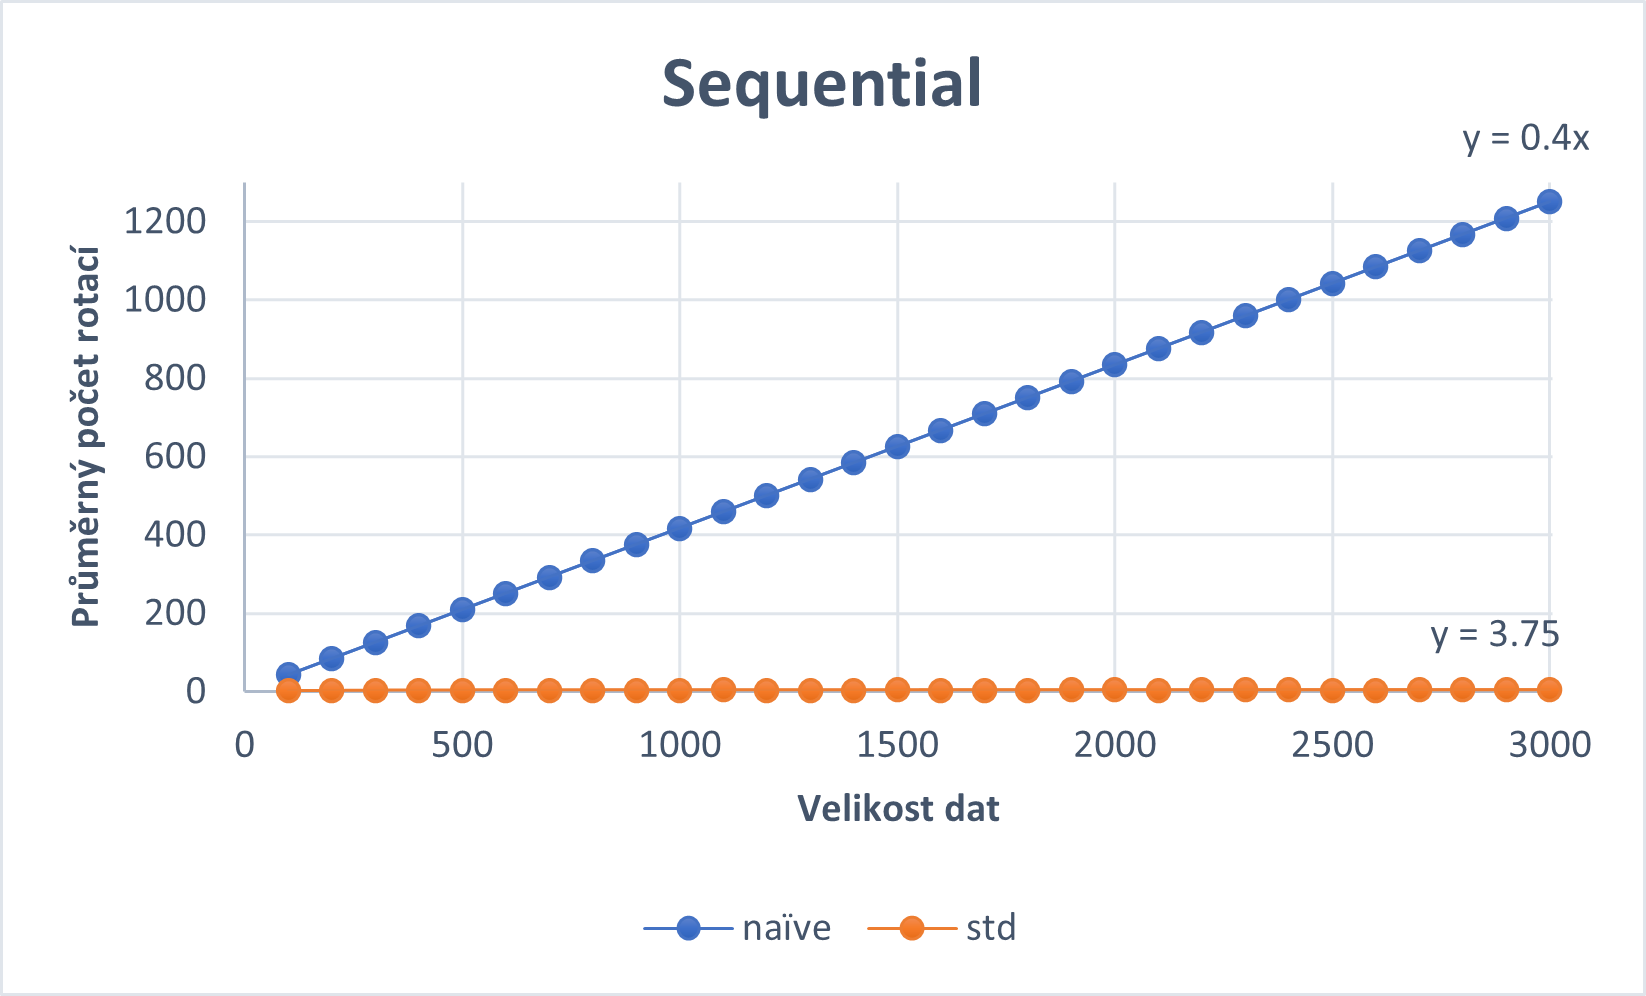
\includegraphics[width=1\textwidth]{img/Sequential.png}
        \caption{Naivní vs správná implementace. Vertikální osa je logaritmická.}
		\label{fig:1_sequential}
	\end{figure}


	\pagebreak
	\subsection{Náhodný přístup}
	Na grafu (Obrázek~\ref{fig:1_random}) pozorujeme u standardního algoritmu logaritmický počet rotací vzhledem k velikosti dat.

	Naivní implementace má řádově stejný počet rotací jako standardní implementace, jen o v průměru cca 10\% lepší,
	což nepovažujeme za výrazný rozdíl.
	\begin{figure}[H]
		\centering
		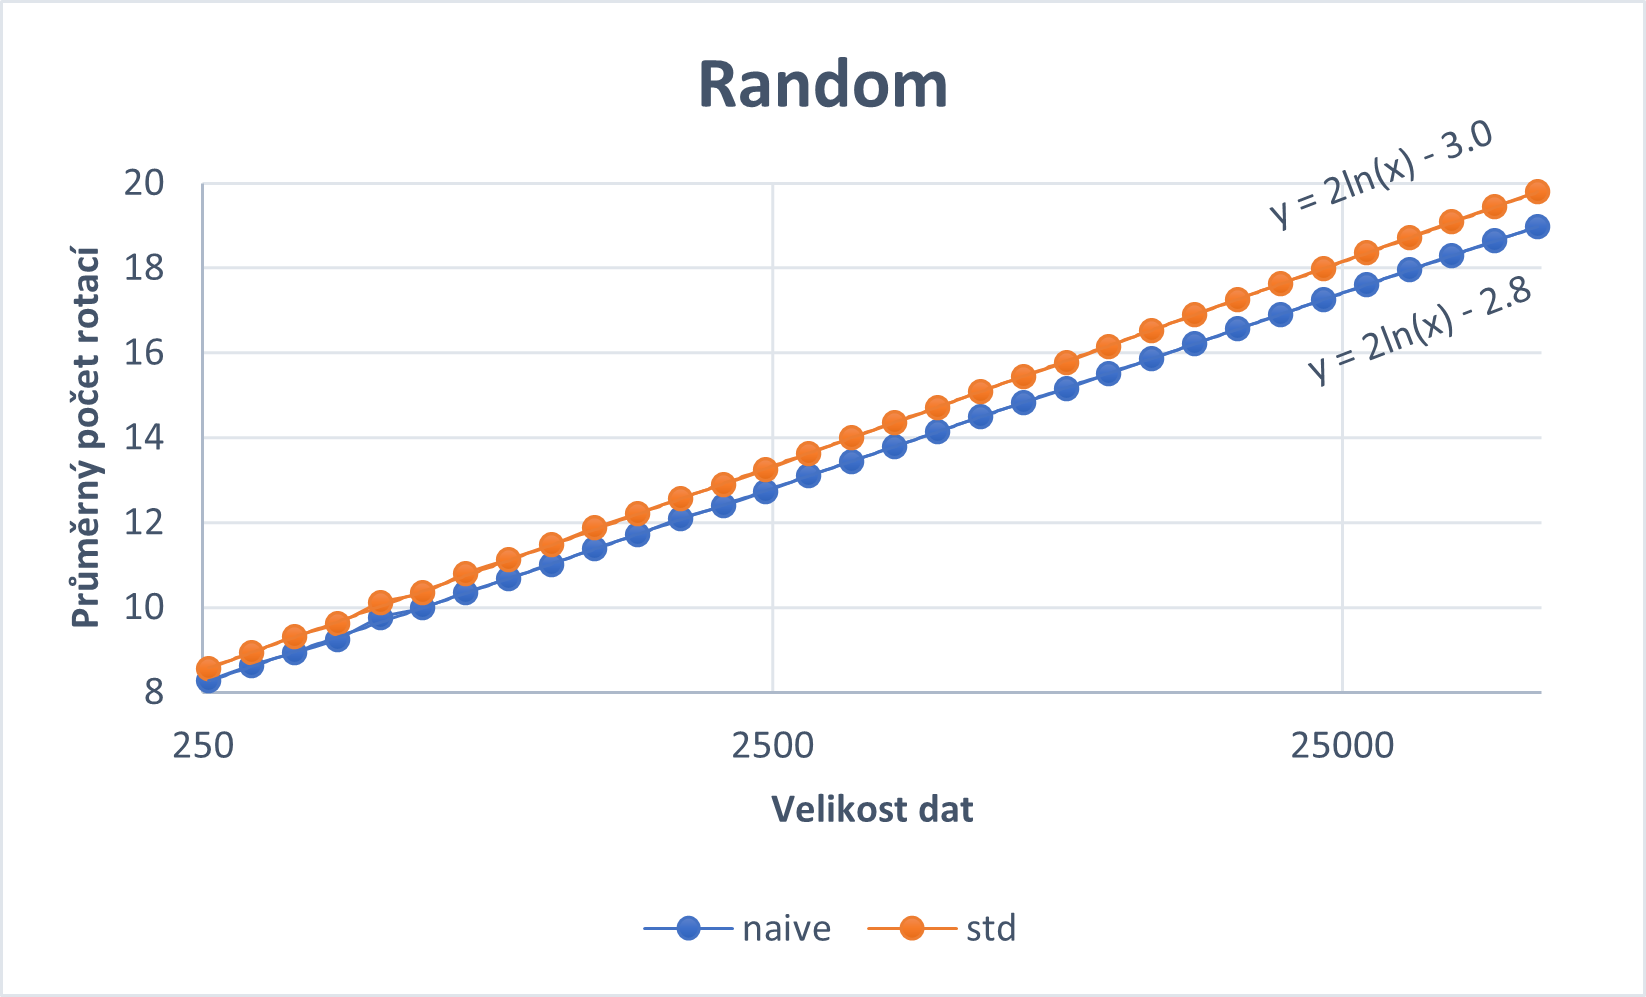
\includegraphics[width=1\textwidth]{img/Random.png}
        \caption{Naivní vs správná implementace. Horizontální osa je logaritmická.}
		\label{fig:1_random}
	\end{figure}


	\pagebreak
	\subsection{Přístup k omezeně velkému výběru prvků}
	Na grafu (Obrázek~\ref{fig:1_subset}) pozorujeme u obou implementací konstantní počet rotací vzhledem k velikosti často přistupavaných dat.

	Takovýto přístup k datům lze srovnávat s nahodným přístupem do dat s konstantní velikostí. 
	\begin{figure}[H]
		\centering
		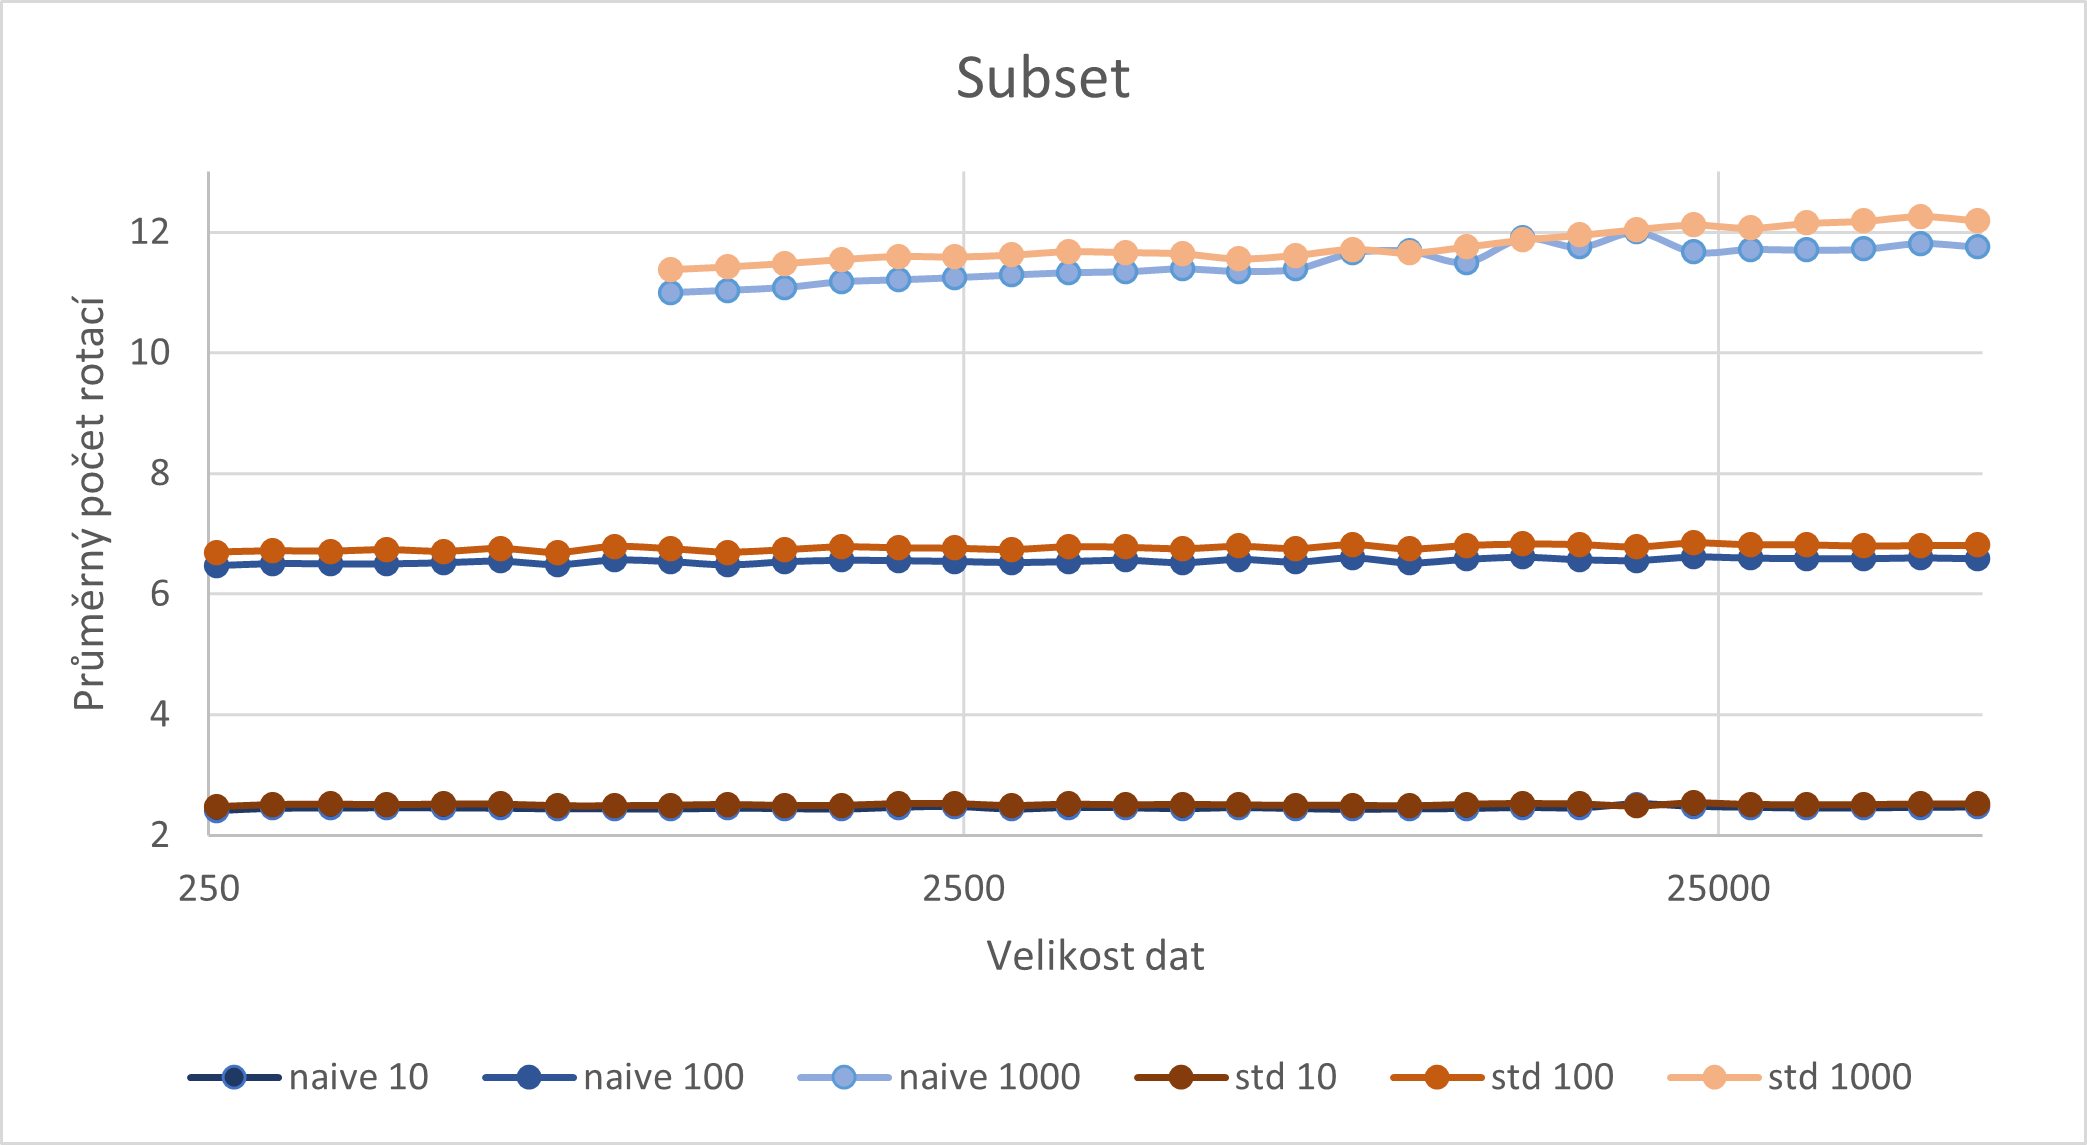
\includegraphics[width=1\textwidth]{img/Subset.png}
        \caption{Naivní vs správná implementace. Horizontální osa je logaritmická.}
		\label{fig:1_subset}
	\end{figure}

	
	\pagebreak
	\section{Měření času}

  	Všechna měření probíhala na stejném zařízení a počet opakování každého testu byl 5.

	Je důležité uvědomit si, že dataset sekvenčního čtení nebyl stejně velký jako ostatní dva datasety, proto jej nemůžme porovnat.

	Náhodné čtení běželo cca dvakrát déle, než přístup do častých dat, což si lze vysvětlit velikostí datasetu, jenž k tomu není reprezentativní a
	pro větší datasety by rozdíl byl větší.

	Sekvenční přístup k datům má očividný rozdíl způsobený porovnáním konstantního přístupu a přísstupu lineárního.	

    \begin{figure}[H]
		\centering
		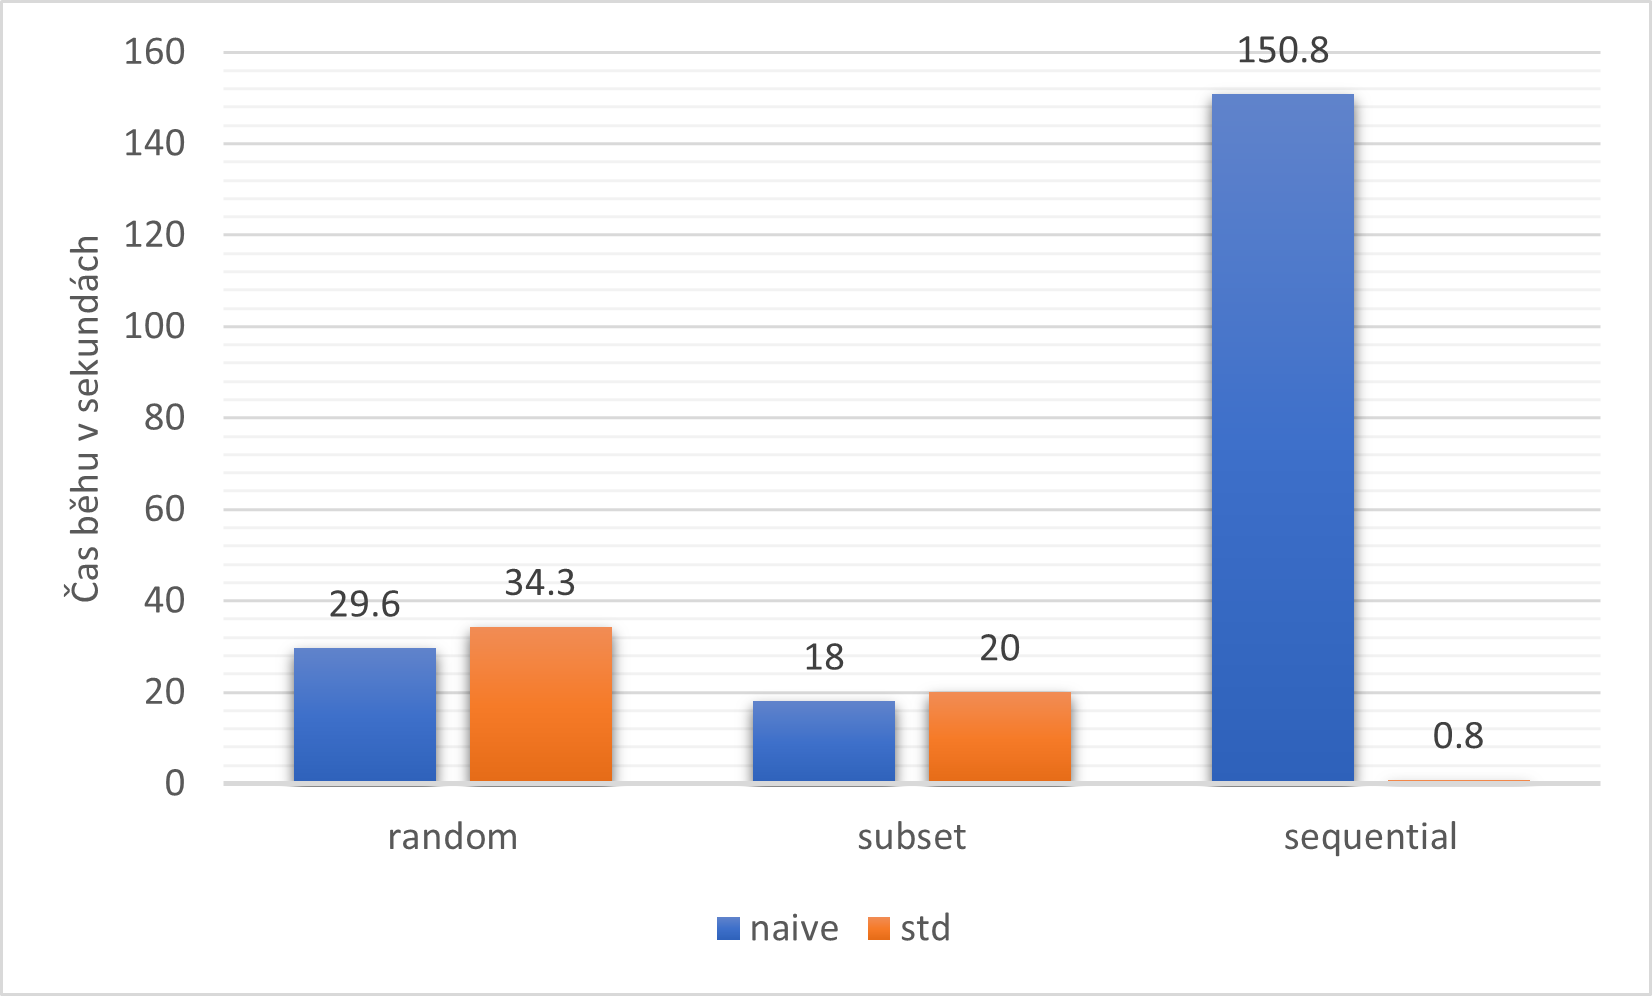
\includegraphics[width=1\textwidth]{img/Time.png}
		\caption{Čas běhu programu.}
		\label{fig:1_time}
	\end{figure}

	
	\subsection{Shrnutí}

	V testech s náhodným přístupem a přístupem do opakujících se dat měly obě implementace řádově stejný počet rotací.

	Jedinou výjimkou byl test sekvenčního hledání, kde standardní implementace měla konstatní počet rotací, avšak naivní lineární.



\end{document}
